% 第二章 摄像机模型与标定

\chapter{摄像机模型与标定}
%------------------------------------------------------------------------------------
\section{摄像机模型}
\subsection{常用坐标系定义及变换}
% ref: 吴哲岑ch2.2,p10; 王德海ch2.1,p9; 王莹ch2.2, p7
% 图像坐标系,摄像机坐标系,世界坐标系
% 图像像素坐标系,图像物理坐标系(成像平面坐标系)
摄像机的成像变换过程涉及到三维的真实世界与二维的图像平面。在视觉测量过程中,世界空间中的点被投影到图像平面上,因此需要定义不同的坐标系并掌握各个坐标系之间的变换方法。常用坐标系包括图像坐标系、成像平面坐标系(也叫图像物理坐标系)、摄像机坐标系和世界坐标系和。

(1)图像坐标系

摄像机采集的图像是以二维(灰度图)或三维(彩色图像)数组的形式储存在计算机中的。设一张图像的分辨率为$M\times N$,则相应得到一个$M\times N$的二维数组,数组中每个元素对应图像中一个像素点。 如图\ref{fig:2_1_image_coord}所示,以图像的左上角为坐标系原点,横轴U指向右、纵轴V指向下,建立直角坐标系$O-UV$,称之为图像坐标系(或图像像素坐标系)。坐标点(u, v)对应图像中第v行第u列的像素。

\begin{figure}[!htb] %图像坐标系和成像平面坐标系
	\centering
	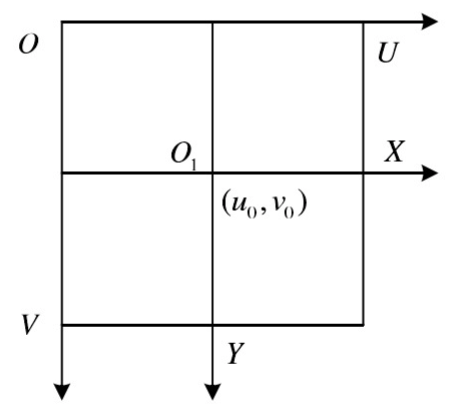
\includegraphics[width=2in]{figures/2_1_image_coord}
	\caption{图像坐标系和成像平面坐标系}\label{fig:2_1_image_coord}
\end{figure}

(2)成像平面坐标系

图像坐标系以像素为基本单位,而现实中以毫米等物理单位来描述物体的尺寸和位置。因此,定义成像平面坐标系$O_1-XY$来建立像素与物理长度之间的联系。在$O_1-XY$坐标系中,定义图像平面与摄像机光轴的交点$O_1$为坐标原点,也称为图像主点。理想情况下,主点位于图像的中心位置,但现实中制造的摄像机会有一定的偏差。坐标轴X、Y轴分别平行于坐标轴U、V。假设主点$O_1$在$O-UV$坐标系中的坐标为$(u_0, v_0)$,每个像素在图像宽和高方向的物理尺寸分别为$d_x$和$d_y$,则图像中某点在成像平面坐标系下的坐标$(x, y)$和图像坐标系下的坐标$(u,v )$之间的关系可表示为:

\begin{equation}\label{eq:2_1_image_coord}
\left\{
	\begin{aligned}
	u&=\frac{x}{d_x}+u_0 \\
	v&=\frac{y}{d_y}+v_0 \\
	\end{aligned}
\right.
\end{equation}

为了便于后面的坐标转换,将其表示成齐次坐标的矩阵形式:
\begin{eqnarray}\label{eq:2_1_image_coord_homogeneous}
\left[\begin{array}{c} u \\ v \\ 1 \end{array} \right]
=
\left[\begin{array}{ccc}
\frac{1}{d_x} & 0 & u_0 \\
0 & \frac{1}{d_y} & v_0 \\
0 & 0 & 1
\end{array}
\right]
\hspace{-6pt} %默认的间距有点大,不知道怎么调整。。
\left[\begin{array}{c} x \\ y \\ 1 \end{array}\right]
\end{eqnarray}

(3)摄像机坐标系

沿摄像机光轴方向移动成像平面坐标系,使坐标原点与光心$O_c$重合,定义Z轴垂直于成像平面坐标系,即摄像机的光轴,从而得到摄像机坐标系$O_c-X_cY_cZ_c$,如图\ref{fig:2_1_camera_and_world_coord}所示。摄像机光心$O_c$到成像平面坐标系原点$O_1$的距离$O_c O_1$即为摄像机的焦距$f$。

\begin{figure}[!htb] %图像坐标系和成像平面坐标系
	\centering
	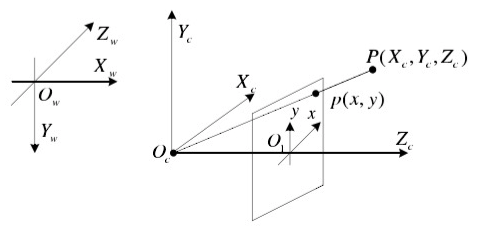
\includegraphics[width=4in]{figures/2_1_camera_and_world_coord}
	\caption{图像坐标系和成像平面坐标系}\label{fig:2_1_camera_and_world_coord}
\end{figure}

(4)世界坐标系

摄像机在三维空间中的位置通常不是固定的,因此更了更方便地描述场景中目标物体的真实位置,需建立一个唯一的世界坐标系$O_w-X_wY_wZ_w$。设场景中任一点在世界坐标系和摄像机坐标系下的坐标分别为$(X_w, Y_w, Z_w)$和$(X_c, Y_c, Z_c)$,则二者之间的转换可以表示为:

\begin{eqnarray}\label{eq:2_1_world_camera_coord_transform}
\left[\begin{array}{c} X_c \\ Y_c \\ Z_c \\ 1 \end{array} \right]
=
\left[\begin{array}{cc}
\mathbf{R} & \mathbf{t}  \\
\mathbf{0^T} & 1
\end{array}
\right]
\hspace{-6pt} %默认的间距有点大,不知道怎么调整。。
\left[\begin{array}{c} X_w \\ Y_w \\ Z_w \\ 1 \end{array}\right]
=\mathbf{M_1}
\hspace{-3pt} 
\left[\begin{array}{c} X_w \\ Y_w \\ Z_w \\ 1 \end{array}\right]
\end{eqnarray}
其中,$\mathbf{R}$和$\mathbf{t}$分别用来描述两坐标系之间的旋转和平移关系,$\mathbf{R}$为$3\times 3$的正交矩阵,$\mathbf{t}$为长度为3的向量,$\mathbf{0_t}=[0, 0, 0]$,$\mathbf{M_1}$为$4\times4$的矩阵。


%------------------------------------------------------------------------------------
\subsection{摄像机线性模型}
% ref: 尚倩ch2.1,p13; 王德海ch2.1, p11; 吴哲岑ch3.1,p19; 苏东ch2.1, p10.
摄像机的线性模型即针孔(pinhole)模型\cite{zhang1999flexible, zhang2000flexible}。在此模型中,来自某一点的光线从物体上发射过来,通过一个平面上的针孔,投射在成像平面上,其余的光束都被针孔平面所阻挡,如图\ref{fig:2_1_pinhole_model}所示。因此物体在图像中的大小只需要一个参数来描述:焦距(focal length),即针孔到成像平面的距离。 设摄像机焦距为$f$,相机到所拍物体的距离为$Z_c$,所拍物体的长度为$X_c$,则利用三角形相似原理可以得到物体在图像上的长度$x$:

\begin{equation}\label{eq:2_1_triangular_similarity}
-x = f \cdot \frac{X_c}{Z_c}
\end{equation}

\begin{figure}[!htb] %摄像机针孔模型
	\centering
	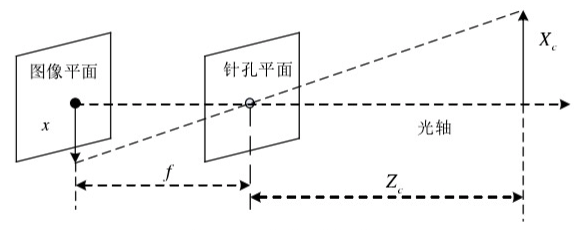
\includegraphics[width=4in]{figures/2_1_pinhole_model}
	\caption{摄像机针孔模型}\label{fig:2_1_pinhole_model}
\end{figure}

负号的存在表示图像中的物体是倒立的。为了略去等式左侧的负号,我们把图像平面放到针孔的右侧,形成了更直观的三角形相似关系$x/f = X_c/Z_c$,图像中的物体由倒立变为了正立。因此,摄像机坐标系下的点$P(X_c, Y_C, Z_C)$在成像平面上的坐标可表示为

\begin{eqnarray}\label{eq:2_1_imaging_plane_and_world_transform}
Z_c
\left[\begin{array}{c} x \\ y \\ 1 \end{array} \right]
=
\left[\begin{array}{cccc}
f & 0 & 0 & 0 \\
0 & f & 0 & 0 \\
0 & 0 & 1 & 0
\end{array}
\right]
\hspace{-6pt} %默认的间距有点大,不知道怎么调整。。
\left[\begin{array}{c} X_c \\ Y_c \\ Z_c \\ 1 \end{array}\right]
\end{eqnarray}

综合式\ref{eq:2_1_image_coord_homogeneous}、\ref{eq:2_1_world_camera_coord_transform}和\ref{eq:2_1_imaging_plane_and_world_transform},可以得到空间中任意一点$P$在世界坐标系和图像坐标系下的坐标转换关系:

\begin{eqnarray}\label{eq:2_1_image_and_world_transform}
Z_c
\left[\begin{array}{c} u \\ v \\ 1 \end{array} \right]
=
\left[\begin{array}{ccc}
\frac{1}{d_x} & 0 & u_0 \\
0 & \frac{1}{d_y} & v_0 \\
0 & 0 & 1
\end{array}\right]
\hspace{-6pt}
\left[\begin{array}{cccc}
f & 0 & 0 & 0 \\
0 & f & 0 & 0 \\
0 & 0 & 1 & 0
\end{array}\right]
\hspace{-6pt}
\left[\begin{array}{cc}
\mathbf{R} & \mathbf{t}  \\
\mathbf{0^T} & 1
\end{array}\right]
\hspace{-6pt}
\left[\begin{array}{c} X_w \\ Y_w \\ Z_w \\ 1 \end{array}\right]
\\
= 
\left[\begin{array}{cccc}
f_x & 0 & u_0 & 0 \\
0 & f_y & v_0 & 0 \\
0 & 0 & 1 & 0
\end{array}\right]
\hspace{-6pt}
\left[\begin{array}{cc}
\mathbf{R} & \mathbf{t}  \\
\mathbf{0^T} & 1
\end{array}\right]
\hspace{-6pt}
\left[\begin{array}{c} X_w \\ Y_w \\ Z_w \\ 1 \end{array}\right]
=
M_1 M_2
\left[\begin{array}{c} X_w \\ Y_w \\ Z_w \\ 1 \end{array}\right]
= M
\left[\begin{array}{c} X_w \\ Y_w \\ Z_w \\ 1 \end{array}\right]
\end{eqnarray}
其中,$f_x=\frac{f}{d_x}$,$f_y=\frac{f}{d_y}$,$f_x, f_y, u_0, v_0$只与摄像机的内部结构有关,为摄像机的内部参数;$\mathbf{R}, \mathbf{t}$描述的是摄像机坐标系与世界坐标系的相对位置关系,为摄像机的外部参数。$M_1$和$M_2$分别称为内参矩阵(intrinsics matrix)和外参矩阵(extrinsics matrix)。对于一部摄像机来说,内部参数是固定不变的,而外部参数可能改变。$M=M_1 M_2$为$3\times 4$的投影矩阵,摄像机将将三维空间中的点映射到二维投影平面上的过程叫作投影变换。

注意到内参$f_x$实际上是透镜的物理焦距长度$f$与成像尺度因子$s_x=\frac{1}{d_x}$的乘积,这样做的意义在于$f$的单位是mm,$s_x$的单位是像素/mm,从而$f_x$的单位是像素。摄像机的标定并不能得到$f$和$s_x$,只有组合量$f_x$和$f_y$可以通过标定直接计算出来。

%------------------------------------------------------------------------------------
\subsection{摄像机非线性模型}
% ref: 白鹏,尚倩,王德海,吴哲岑.
针孔模型只是一个理想的模型,而实际情况下通过光心的光线太少会导致曝光不足,图像生成缓慢。因此我们生活中使用的摄像机都利用透镜来使足够多的光线收敛聚焦到成像平面上\cite{GaryBradski2009学习}。理论上可以定义不造成任何畸变的透镜,但现实中由于制造工艺问题,所有透镜都存在一定程度的畸变。为了获得较为精确的摄像机模型,需要对畸变进行建模。

摄像机的畸变主要有径向畸变(radial distortions)\cite{hartley2003multiple}、离心畸变(decentering distortions)\cite{ricolfe2010lens}和薄棱镜畸变(thin prism distortions)\cite{weng1992camera}。第一种主要是由棱镜的形状缺陷导致的,其只会造成径向位置误差;后两种主要是由棱镜和相机的不当安装导致的,其同时会造成径向和切向的位置误差\cite{weng1992camera}。

我们可以使用一组数学表达式来表示畸变,在摄像机的线性模型基础上加入畸变的表达式,得到一个摄像机的非线性模型。非线性畸变可表示为式\ref{eq:2_1_lens_distortion}的形式。

\begin{equation}\label{eq:2_1_lens_distortion}
\left\{
\begin{aligned}
x' &= x + \sigma_x (x,y)  \\
y' &= y + \sigma_y(x,y)
\end{aligned}
\right.
\end{equation}
其中,$(x,y)$是线性模型计算得到的成像平面坐标系下的坐标,$(x',y')$是计入畸变后更准确的坐标,$\sigma_x$和$\sigma_y$是非线性模型中的畸变参数。

(1)径向畸变

径向畸变又称径向失真,主要是由棱镜的径向曲率曲线的缺陷造成的。径向畸变可分为两类,符号为负的径向位移被称为桶形畸变(barrel distortion),它会使距离光心远的点挤向一起;符号为正的径向位移被称为枕形畸变(pincushion),它会使距离光心远的点更加分散。这种畸变关于光轴是严格对称的,我们可以用泰勒展开式来对径向畸变建模,如式\ref{eq:2_1_radial_distortion}。试验表明,使用$k1$和$k2$两项即可校正90\%以上的径向畸变\cite{hartley2003multiple}。

\begin{equation}\label{eq:2_1_radial_distortion}
\left\{
\begin{aligned}
\sigma_x(x,y) &= x(k_1 r^2 + k_2 r^4 + k_3 r^6 + \cdots)  \\
\sigma_y(x,y) &= y(k_1 r^2 + k_2 r^4 + k_3 r^6 + \cdots) 
\end{aligned}
\right.
\end{equation}

\begin{figure}[!htb] %桶形畸变和枕形畸变
	\centering
	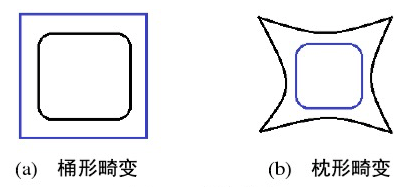
\includegraphics[width=4in]{figures/2_1_radial_distortion}
	\caption{桶形畸变和枕形畸变系}\label{fig:2_1_radial_distortion}
\end{figure}

(2)离心畸变

离心畸变是镜头各部件的光心不严格共线造成的,现实中的光学系统都存在不同程度的离心畸变。这种畸变可描述为式\ref{eq:2_1_decentering_distortion}。

\begin{equation}\label{eq:2_1_decentering_distortion}
\left\{
\begin{aligned}
\sigma_x(x,y) &= 2p_2 xy + p_1 (3x^2 + y^2)  \\
\sigma_y(x,y) &= 2p_1 xy + p_2 (x^2+ 3y^2)
\end{aligned}
\right.
\end{equation}

(3)薄棱镜畸变

薄棱镜畸变是由透镜的设计、生产和相机装配中的缺陷造成的,例如透镜光轴与摄像机的面阵平面之间存在微小的倾斜。这种畸变可使用式\ref{eq:2_1_thin_prism_distortion}来表示。

\begin{equation}\label{eq:2_1_thin_prism_distortion}
\left\{
\begin{aligned}
\sigma_x(x,y) &= s_1 (x^2 + y^2) \\
\sigma_y(x,y) &= s_2 (x^2 + y^2)
\end{aligned}
\right.
\end{equation}

三种畸变中,径向畸变是最主要的畸变成分,薄棱镜畸变的影响很小,可忽略不计。因此,综合径向畸变和离心畸变,透镜畸变模型可表示为:

\begin{equation}\label{eq:2_1_radial_distortion}
\left\{
\begin{aligned}
\sigma_x(x,y) &= x(k_1 r^2 + k_2 r^4) + (2p_2 xy + p_1 (3x^2 + y^2))  \\
\sigma_y(x,y) &= y(k_1 r^2 + k_2 r^4)  + (2p_1 xy + p_2 (x^2 + 3y^2))
\end{aligned}
\right.
\end{equation}


%------------------------------------------------------------------------------------
\section{摄像机标定}
摄像机标定就是确定其内部参数和外部参数的过程。
\subsection{单目摄像机标定}
\subsection{双目摄像机标定}

\section{双目立体视觉原理}

\section{实验结果}

\section{本章小结}
